\documentclass[resume]{subfiles}


\begin{document}
\section{Causal Loop Diagrams}
\begin{itemize}
\item Capturer les hypothèses sur les causes du
  comportement dynamique d'un système
\item Révélez nos "modèles mentaux"
\item Implanter les éléments de rétroaction dans nos modèles  
\end{itemize}

Si nombre de lien - paire alors boucle + sinon -
\begin{figure}[H]
    \centering
    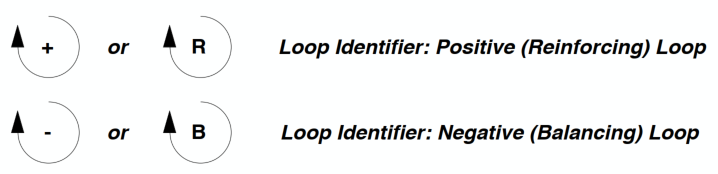
\includegraphics[width=0.8\columnwidth]{Figures/CLD_1.PNG}
    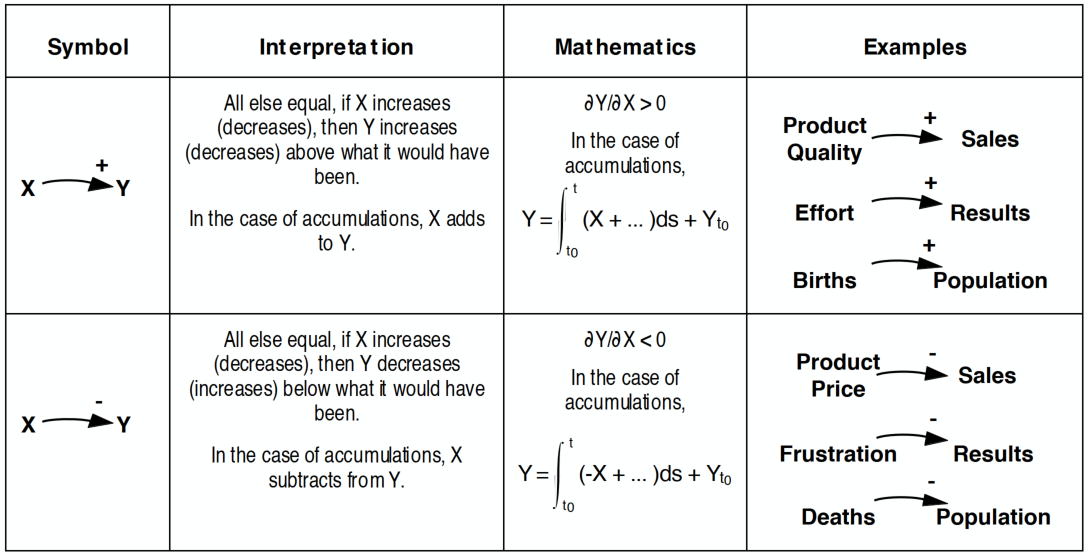
\includegraphics[width=0.8\columnwidth]{Figures/CLD_2.PNG}
\end{figure}

\subsubsection{A faire attention}
\begin{itemize}
\item Si il y a une ambiguïté sur le signe de la flèche c'est qu'il manque une étape
\item Des noms plutôt que des phrases (X,Y)
\item Les noms de variables doivent avoir un sens en
  cohérence la sensibilité
\item Choisir les labels dont l'évolution est normalement
  espérée ou mesurée > 0
\end{itemize}

\subsection{Stock and Flow}

\subsubsection{Stocks}
\begin{itemize}
\item CLD ne représentent pas l'accumulation, les Stocks oui
\item Stocks = état du système (et nos décisions dépendent de
  l'état)
\item E.G.: l'inventaire d'une entreprise, le \# d'employés, le
  montant sur le compte de paiements  
\end{itemize}

\subsubsection{Flow}
\begin{itemize}
\item Les flux changent les stocks
  \item L'inventaire change avec les livraisons
  \item \# d'employés ch ange avec les recrutements, licenciements et départs à la retraite
\item Souvent, on a des problèmes à décider comment
  distinguer flux et taux (l'inflation?)  
\end{itemize}
\begin{figure}[H]
    \centering
    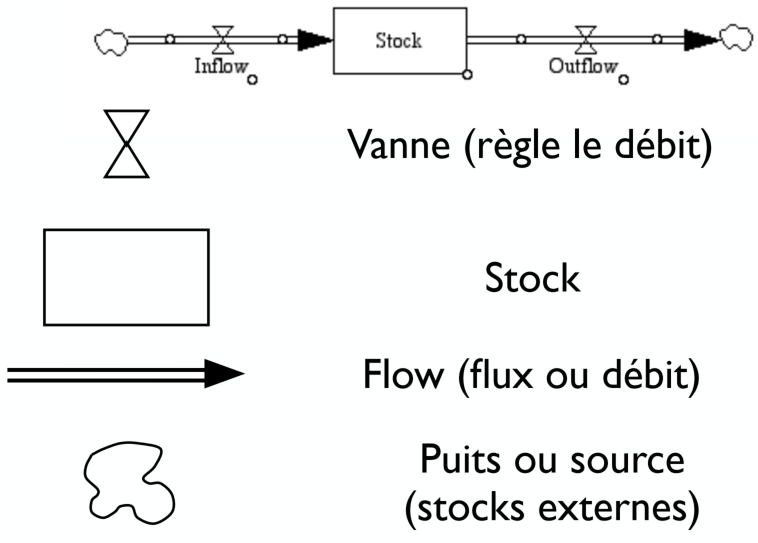
\includegraphics[width=0.8\columnwidth]{Figures/StockFlow.PNG}
\end{figure}


\subsection{Math}

Les niveaux (stocks) intègrent les débits (flows)

$stock(t)=\int^t_{t_0}[in(s)-out(s)]ds + stock(t_0)$ ceci donne $\frac{d(stock)}{dt}=in(t)-out(t)$ 

\end{document}